\section{Iteración V}
\subsection{Resumen}
En esta iteración desarrollamos la función \textbf{ARFRecoverAccount} para implementar un proceso seguro de recuperación de la contraseña de una cuenta en caso de haberla olvidado.

\subsection{Desarrollo}
El método cumple la regla de negocio \textbf{BR3} y sigue el proceso de negocios mostrado en la figura 4.35.
\begin{figure}[h!]
	\centering
	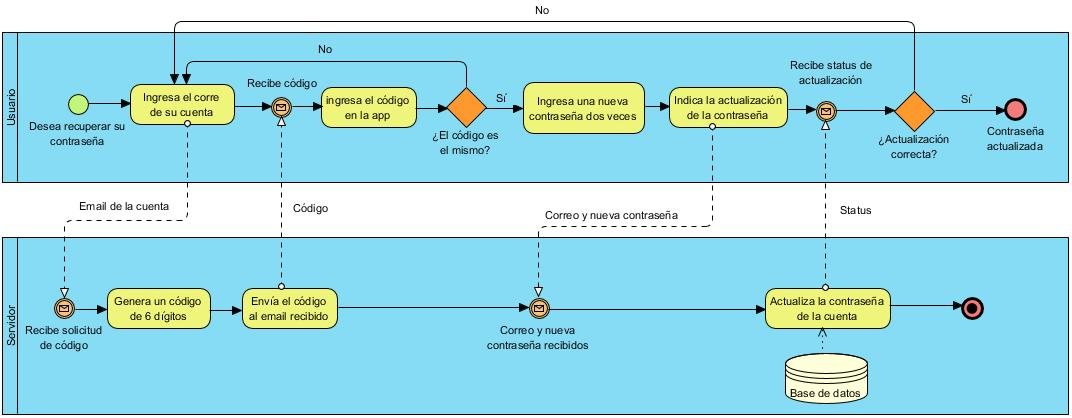
\includegraphics[width=15cm,height=6cm]{imagenes/desarrollo/diagramas/BPMN_RECOVER.jpg}
	\caption{Diagrama de proceso de recuperación de contraseña.}
	\label{fig:recover}
\end{figure}

A nivel aplicativo consta de tres pasos, cada uno con sus respectivas pantallas:
\begin{itemize}
	\item El usuario ingresa el email de su cuenta de la cual quiere recuperar la contraseña (ver figura 4.36)
	\item El sistema genera y envía un código al email de la cuenta. El usuario deberá escribir este código en la aplicación para verificar que tiene acceso al correo y así validar que efectivamente sea su cuenta (ver figura 4.37).
	\item El usuario escribe una nueva contraseña y la guarda para sustituir a la contraseña anterior (ver figura 4.38).
\end{itemize}


\begin{figure}[h!]
	\begin{minipage}{0.32\textwidth}
		\centering
		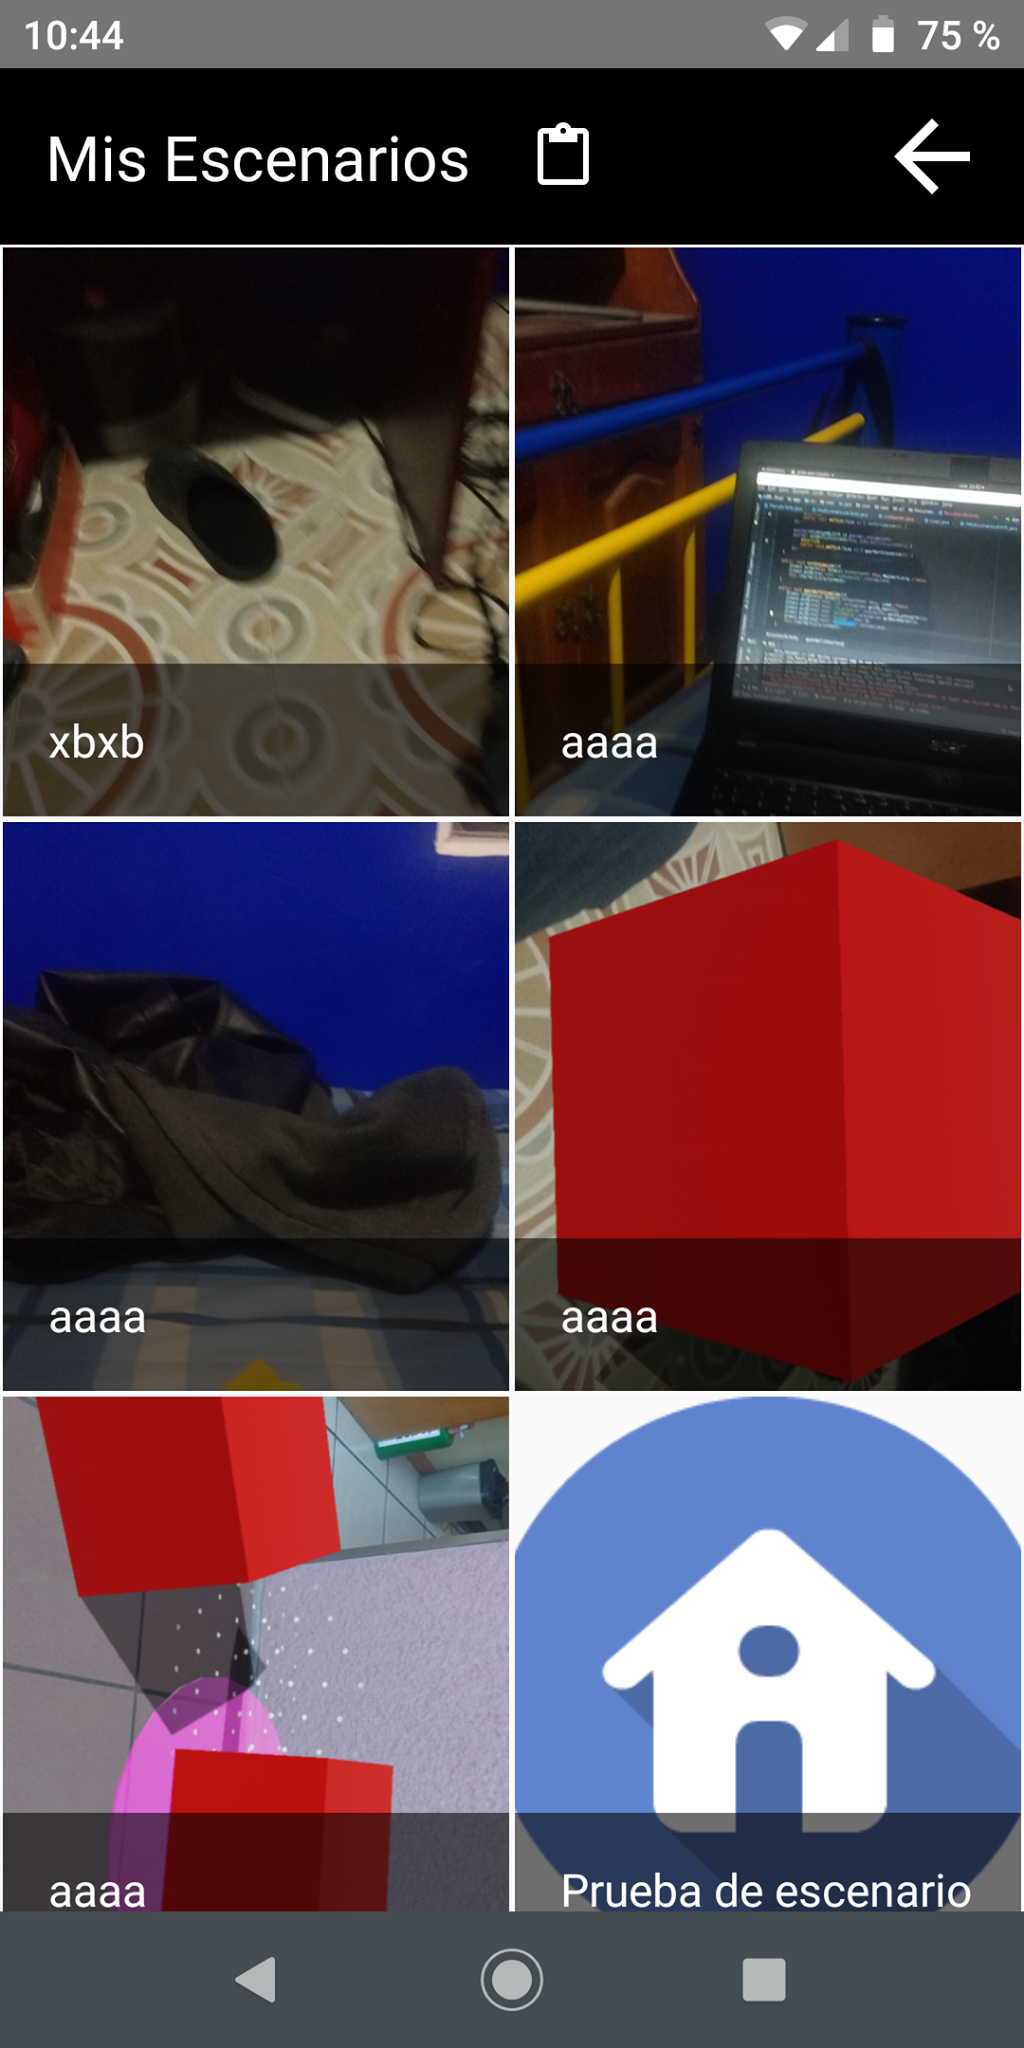
\includegraphics[width=4cm,height=8cm]{imagenes/desarrollo/app/scenarios.png}
		\caption{Visualización de proyectos}
		\label{fig:rec02}
	\end{minipage}\hfill
	\begin{minipage}{0.32\textwidth}
		\centering
		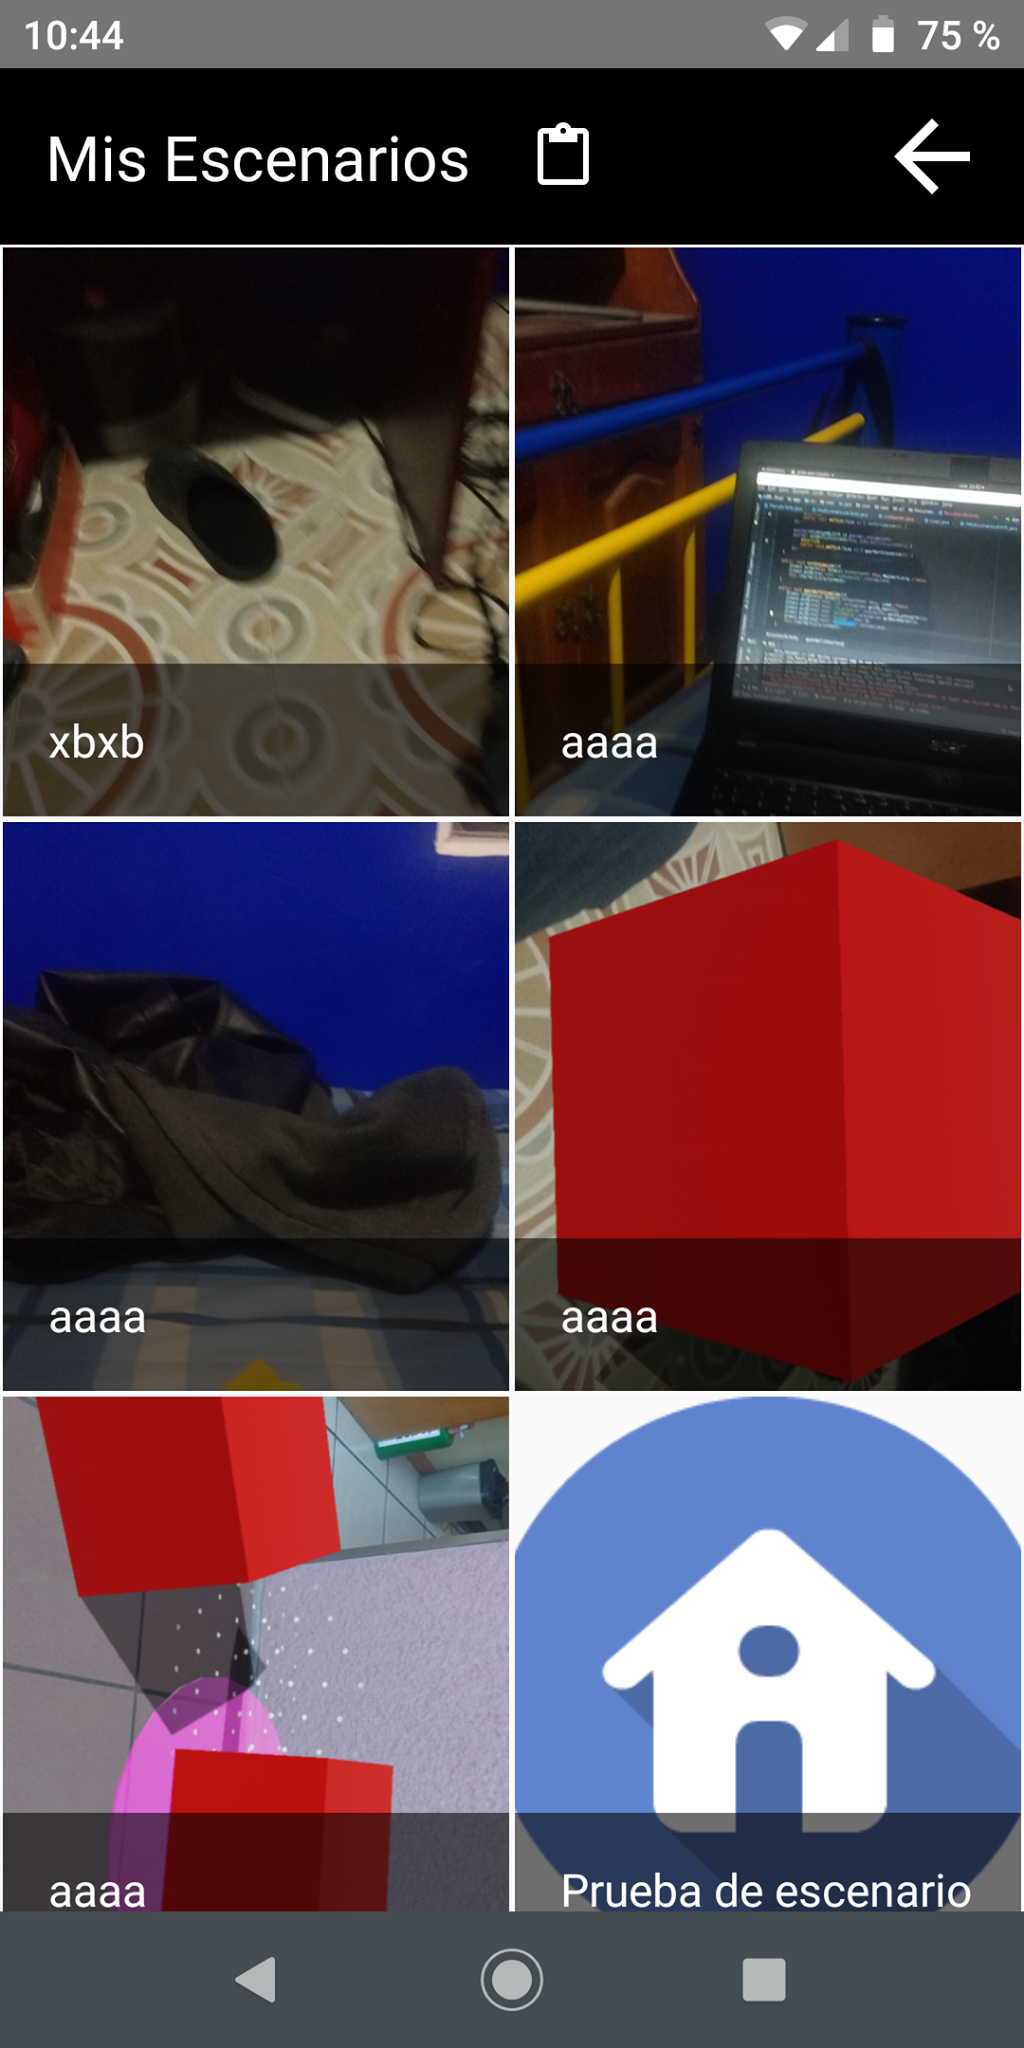
\includegraphics[width=4cm,height=8cm]{imagenes/desarrollo/app/scenarios.png}
		\caption{Actualización de proyecto}
		\label{fig:rec01}
	\end{minipage}\hfill
	\begin{minipage}{0.32\textwidth}
		\centering
		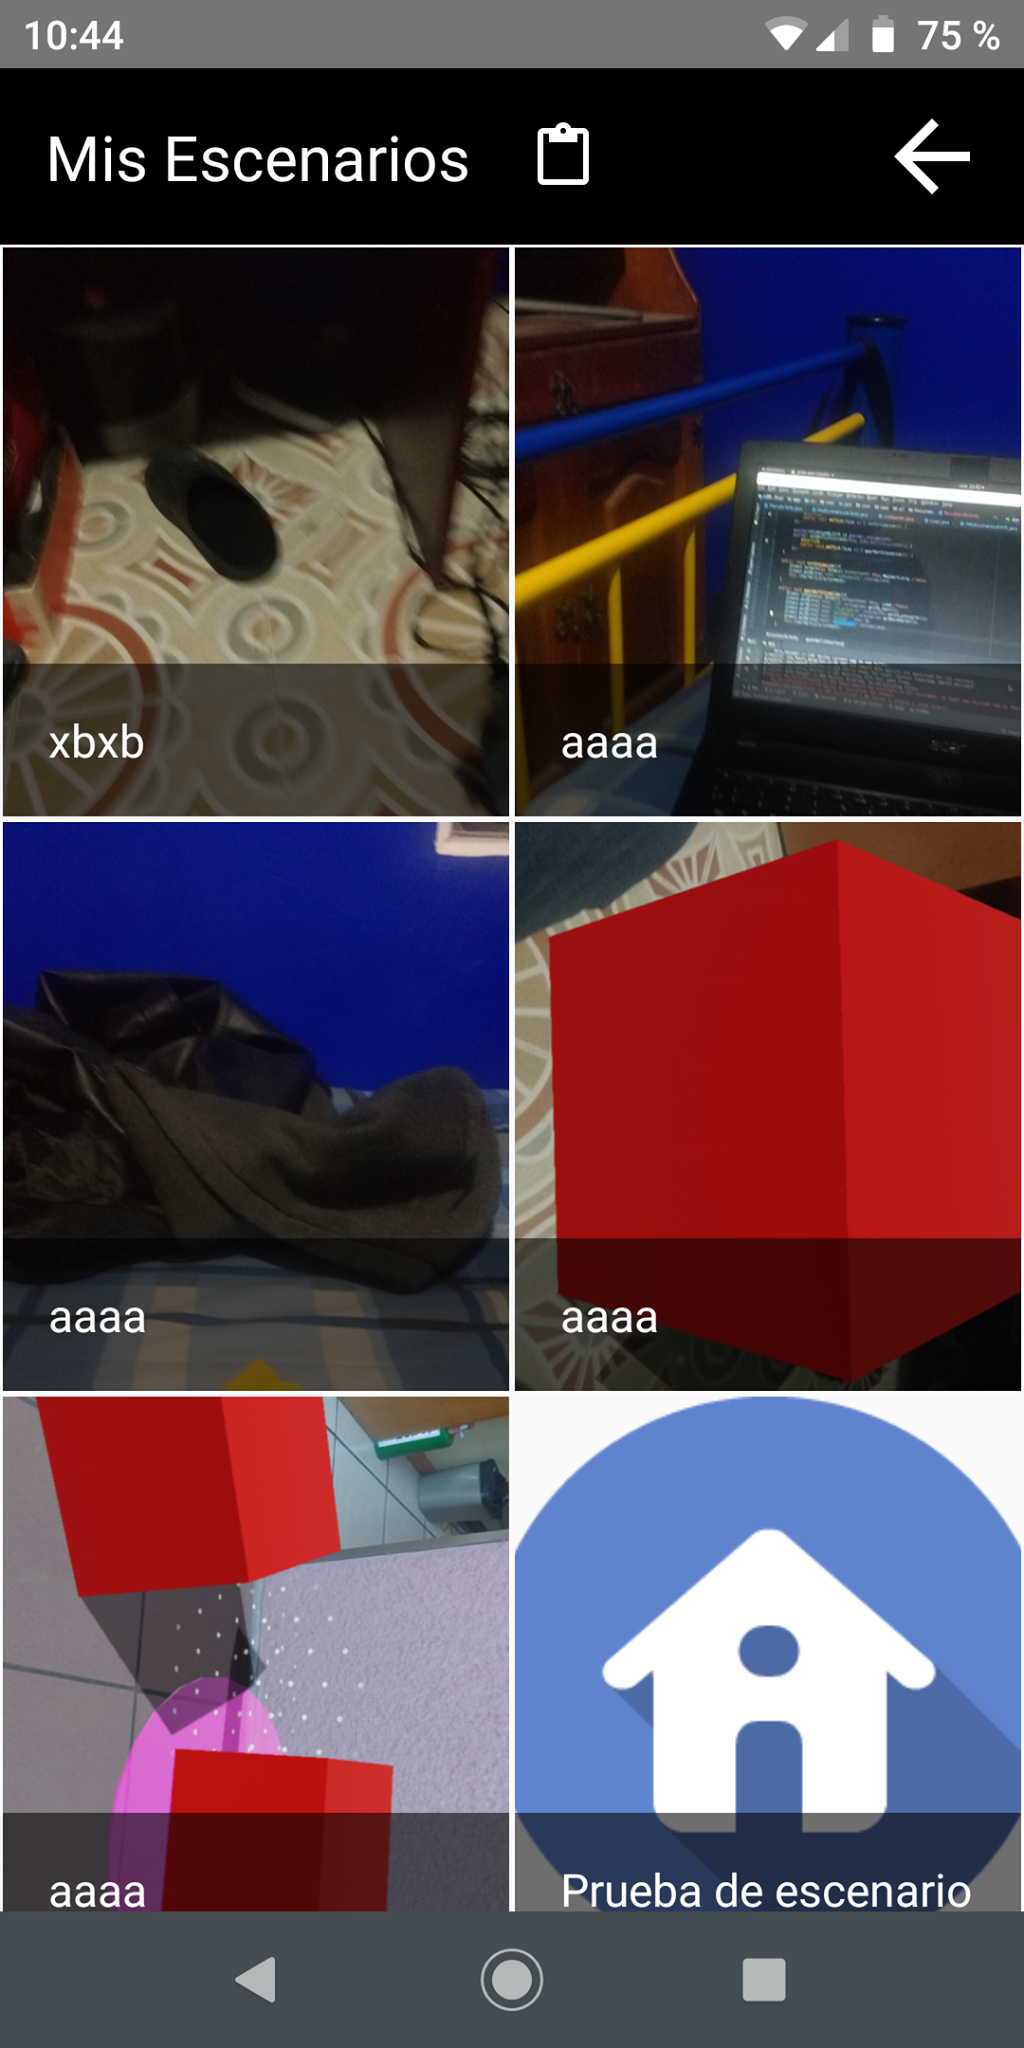
\includegraphics[width=4cm,height=8cm]{imagenes/desarrollo/app/scenarios.png}
		\caption{Agregar nueva proyecto}
		\label{fig:rec03}
	\end{minipage}\hfill
\end{figure}

\clearpage
